\documentclass[xcolor=dvipsnames]{beamer}
\usepackage[spanish,activeacute]{babel}
\usepackage[utf8]{inputenc}
\usepackage{listings}
\usepackage{amsmath,amsfonts,amssymb}
\usepackage{adjustbox}
\usepackage{color}
\usepackage{tikz}
\usetikzlibrary{shapes,arrows}
\usepackage{multicol}
%\usepackage{slashbox,pict2e}
\usepackage{pgf}
\usepackage{algorithm} %REVISAR FORMATO DE ALGORITMO
\usepackage{algorithmic}
\renewcommand{\algorithmicrequire}{\textbf{Input:}}
\renewcommand{\algorithmicensure}{\textbf{Output:}}
\def\R{{\mathbb R }}
\def\N{{\mathbb N }}
\usetheme{Warsaw}
%\usecolortheme{lily}
%\usecolortheme{beaver}


\definecolor{myblue1}{RGB}{35,119,189}
\definecolor{myblue2}{RGB}{95,179,238}
\definecolor{myblue3}{RGB}{129,168,207}
\definecolor{myblue4}{RGB}{26,89,142}

\setbeamercolor*{structure}{fg=myblue1,bg=blue}
\setbeamercolor*{palette primary}{use=structure,fg=white,bg=structure.fg}
\setbeamercolor*{palette secondary}{use=structure,fg=white,bg=structure.fg!75!black}
\setbeamercolor*{palette tertiary}{use=structure,fg=white,bg=structure.fg!50!black}
\setbeamercolor*{palette quaternary}{fg=black,bg=white}
\setbeamercolor*{item projected}{fg=red,bg=myblue3!80}
\setbeamercolor*{block title example}{fg=white,bg=myblue4}
\setbeamercolor*{frametitle}{fg=black}

\setbeamertemplate{blocks}[rounded][shadow=true]

\makeatletter
\pgfdeclarehorizontalshading[frametitle.bg,frametitle right.bg]{beamer@frametitleshade}{\paperheight}{%
  color(0pt)=(myblue2);
  color(\paperwidth)=(white)}

\defbeamertemplate*{footline}{mysplit theme}
{%
  \leavevmode%
  \hbox{\begin{beamercolorbox}[wd=.5\paperwidth,ht=2.5ex,dp=1.125ex,leftskip=.3cm plus1fill,rightskip=.3cm]{author in head/foot}%
    \usebeamerfont{author in head/foot}\insertshortauthor
  \end{beamercolorbox}%
  \begin{beamercolorbox}[wd=.5\paperwidth,ht=2.5ex,dp=1.125ex,leftskip=.3cm,rightskip=.3cm plus1fil]{title in head/foot}%
    \usebeamerfont{title in head/foot}\insertshorttitle\hfill
    \insertframenumber/\inserttotalframenumber\hspace*{0.5em}
  \end{beamercolorbox}}%
  \vskip0pt%
}
\makeatother







\tikzstyle{startstop} = [rectangle, rounded corners, minimum width=3cm, minimum height=1cm,text centered, draw=black, fill=red!30]
\tikzstyle{io} = [trapezium, trapezium left angle=70, trapezium right angle=110, minimum width=3cm, minimum height=1cm, text centered, draw=black, fill=blue!30]
\tikzstyle{process} = [rectangle, minimum width=4cm, minimum height=1cm, text centered, text width=5cm, draw=black, fill=orange!30]
\tikzstyle{decision} = [diamond, minimum width=2cm, minimum height=1cm, text centered, draw=black, fill=green!30]
\tikzstyle{arrow} = [thick,->,>=stealth]



\author[P. Arce et al.]{Paola
Arce\inst{1}\and Jonathan Antognini\inst{1}\and Werner Kristjanpoller
\inst{2}\and Luis Salinas\inst{1,3}}

\institute[UTFSM]{
\inst{1} Departamento de Inform\'atica, UTFSM, Chile \\
\inst{2} Departamento de Industrias, UTFSM, Chile \\
\inst{3} CCTVal, UTFSM, Chile
}

\date[ICPRAM 2015]{4th International Conference on Pattern Recognition
Application and Methods 2015}
\title[Online VECM for FOREX rates forecasting]{\Large An Online Vector Error Correction Model for
Exchange Rates Forecasting}


\titlegraphic{
   \includegraphics[width=1cm]{img/logo_DI}\hspace*{2.5cm}~%
   \includegraphics[width=1.5cm]{img/logo_UTFSM}\hspace*{2.5cm}~%
   \includegraphics[width=1cm]{img/logo_IND}
}

\begin{document}
\begin{frame}[plain]
\titlepage
\end{frame}

\begin{frame}
\frametitle{Outline}
\begin{itemize}
\item Motivation: economic relations
\item Cointegration and Integration concepts
\item VECM model
\item Proposal
\item Experiments
\item Conclusions
\end{itemize}
\end{frame}

\section{Introduction}
\subsection{Motivation}
\begin{frame}
\frametitle{Motivation}
Financial time series are mainly non-stationary.  However, one or more linear
combinations of non-stationary time series can be stationary even though
individually they are not. 


\begin{center}
\includegraphics[width=0.5\textwidth]{img/allcurrencies}
\end{center}
\end{frame}

\begin{frame}
When this happens it is said they have a long-run
equilibrium relationship and the variables are \textbf{cointegrated}.
\end{frame}



\section{Background}
\subsection{Definitions}
\begin{frame}
\frametitle{Integration }
\begin{block}{Integration of order $d$}
A time series $\mathbf{y}$ is said to be integrated of order $d$ if after
differentiating the variable $d$ times, we get an stationary process, more precisely:

\[
(1-L)^d \mathbf{y} \sim \text{I(0)} \, ,
\]

\noindent where I(0) is a stationary time series and $L$ is the lag operator:

\[
(1-L)\mathbf{y} = \Delta \mathbf{y}=\mathbf{y}_t  -\mathbf{y}_{t-1} \quad \forall t
\]
\end{block}
\end{frame}

\subsection{Integration example}
\begin{frame}
\frametitle{Financial Time Series}
\begin{columns}
\column[t]{5cm}
Financial time series are commonly a I(1) process 
\begin{center}
\includegraphics[width=0.85\textwidth]{img/EURUSD}
\end{center}
\column[t]{5cm}
Since their differences are stationary (I(0) process).
\begin{center}
\includegraphics[width=0.85\textwidth]{img/DEURUSD}
\end{center}
\end{columns}
\end{frame}

\subsection{Cointegration}
\begin{frame}
\frametitle{Cointegration}
\begin{block}{Cointegration definition}
Let $\mathbf{y} = \{\mathbf{y}^1, \dots, \mathbf{y}^l\}$ be a set of $l$
time series of order I(1) which are said to be cointegrated if a vector
$\beta=[\beta(1),\dots,\beta(l)]^\top \in \mathbb{R}^l$  exists such that the
time series,

\begin{equation*}
 \mathbf{Z}_t:= \beta^\top \mathbf{y} = \beta(1) \mathbf{y}^1 + \dots + \beta(l) \mathbf{y}^l \sim
 \text{I(0)}\, .
\end{equation*}
\end{block}
In other words, a set of I(1) variables is said to be cointegrated if
a linear combination of them exists which is I(0).

\end{frame}

\subsection{Vector Autorregresive models}
\begin{frame}
\frametitle{VECM: Vector Error Correction model}

VECM is a special form of a Vector Autorregresive model (VAR) for I(1)
variables $\mathbf{y}$ that are also cointegrated. Let 

\begin{equation*}
\label{eq:variables}
\mathbf{y}_t = 
\begin{bmatrix} y_{1,t} & y_{2,t} & \dots & y_{l,t}
\end{bmatrix}^\top \, \qquad t=p+1, \dots N. 
\end{equation*}

\begin{block}{VAR}
VAR($p$) model describes the behaviour of a set of $l$
endogenous variables as a linear combination of their last $p$ values:
{\color{blue}
\begin{equation*}
\label{eq:var}
 \mathbf{y}_t = \phi_1 \mathbf{y}_{t-1}  + \dots +   \phi_p\mathbf{y}_{t-p}
+ \mathbf{c} + \mathbf{\epsilon}_t \, ,
\end{equation*}}
\noindent where  ${\phi_1,\dots,\phi_p}$ are $l \times l$
matrices of real coefficients,
$\mathbf{\epsilon}_{p+1},\dots,\mathbf{\epsilon}_N$ are error terms,
$\mathbf{c}$ is a constant vector and $N$ is the total number of samples.
\end{block}
\end{frame}



\begin{frame}
\frametitle{VECM: Vector Error Correction model}
\begin{block}{VECM}

It is obtained by replacing the form {\color{red} $\Delta
\mathbf{y}_t = \mathbf{y}_t - \mathbf{y}_{t-1}$} in the VAR form.
{\color{blue}
\begin{equation}
 \label{eq:vec}
 \Delta \mathbf{y}_t = 
 \underbrace{ \Omega\mathbf{y}_{t-1}}_\text{Error correction term} + 
 \sum_{i=1}^{p-1}
\phi_i^* \Delta \mathbf{y}_{t-i}  + \mathbf{c} + \mathbf{\epsilon}_t \quad ,
\end{equation}}
\end{block}

\noindent where 
%coefficients matrices $\Omega$ and $\phi_i^*$ are
%function of matrices $\phi_i$ as follows:

\begin{eqnarray*}
\phi_i^* &: =& -\sum_{j=i+1}^{p} \phi_j \\
\Omega &: =& -(\mathbb{I}-\phi_1-\dots-\phi_p) 
\end{eqnarray*}
\end{frame}

\begin{frame}
\frametitle{$\Omega$ matrix properties}
The matrix $\Omega$ has the following properties:
\begin{itemize}
\item If $\Omega = 0$ there is no cointegration
\item If $rank(\Omega)=l$ i.e full rank, then the time series are not
I(1) but stationary
\item If $rank(\Omega)=r,\quad 0 < r < l$ then, there is cointegration
and the matrix $\Omega$ can be expressed as $\Omega =
\alpha \beta^\top$, where $\alpha$ and $\beta$ are $(l \times r)$
matrices and $rank(\alpha)=rank(\beta)=r$.
\end{itemize}
The columns of $\beta$ contains the cointegration vectors and the rows of
$\alpha$ correspond with the adjusted vectors. $\beta$ is obtained by Johansen
procedure whereas $\alpha$ has to be determined as a
variable in the VECM.
\end{frame}


\begin{frame}
\frametitle{VECM matrix form}
\small
\begin{equation*}
\underbrace{
      \begin{bmatrix}
       \mathbf{\Delta y}_{p+1}  \\ 
       \mathbf{\Delta y}_{p+2}  \\ 
       \vdots                   \\ 
       \mathbf{\Delta y}_N      
      \end{bmatrix}}_{\mathbf{B} } =
\arraycolsep=1.4pt  
\underbrace{\begin{bmatrix}
   \alpha^\top & \phi^*_1 & \dots & \phi^*_{p-1} &\mathbf{c}   
  \end{bmatrix}}_{\mathbf{X}^\top}
\underbrace{\begin{bmatrix}
 \beta\mathbf{y}_p      & \beta\mathbf{y}_{p+1}   & \dots&   \beta\mathbf{y}_{N-1}   \\
 \mathbf{\Delta y}_{p}   & \mathbf{\Delta y}_{p+1}& \dots &  \mathbf{\Delta y}_{N-1} \\
 \mathbf{\Delta y}_{p-1} & \mathbf{\Delta y}_{p}  & \dots &  \mathbf{\Delta y}_{N-2}   \\
 \vdots                  & \vdots                 & \ddots&  \vdots                   \\
 \mathbf{\Delta y}_{2}   & \mathbf{\Delta y}_{3} & \dots &   \mathbf{\Delta y}_{N-p+1} \\
 1                      & 1                       & \dots     & 1   
 \end{bmatrix}}_{\mathbf{A}^\top}
+
\underbrace{\begin{bmatrix}
              \mathbf{\epsilon}_{p+1} \\ 
              \mathbf{\epsilon}_{p+2} \\ 
              \vdots \\ 
              \mathbf{\epsilon}_N
             \end{bmatrix}}_{\mathbf{E}^\top}
\end{equation*}
\end{frame}

\begin{frame}
\frametitle{VECM difficulties}
\begin{itemize}
\item VECM parameter estimation is done by the Johansen method and OLS which are
computationally expensive routines.
\item VECM parameters must be recalculated every time new data is available. 
\end{itemize}
\end{frame}

\section{Experiments}
\subsection{Proposal}
\begin{frame}
\frametitle{Proposal: Online VECM algorithm (OVECM)}
\begin{itemize}
\item Considers only a sliding window of the $L$ most recent data. 
\item Since cointegration vectors represent long-run relationships they vary
little in time. OVECM obtains these vectors only when they need to be updated. 
\item This updating is done when MAPEs of the last $n$ inputs is above a certain
error given by a threshold 
\item OVECM also implements matrix optimisations in order to reduce execution time,
such as updating matrices with new data, removing old data and introducing new
cointegration vectors.
\end{itemize}
\end{frame}


%\begin{frame}
%\begin{center}
%    \begin{adjustbox}{max size={.95\textwidth}{.8\textheight}} %height=0.8\textheight}
%    \begin{tikzpicture}[node distance=2cm]
%    %\node (start) [startstop] {Start};
%    %\node (in1) [io, below of=start] {Input};
%    \node (in1) [io] {Input: y, p, L, $\epsilon$, n};
%    \node (pro1) [process, below of=in1] {$y_i = y[i:i+L]$};
%    \node (dec1) [decision, below of=pro1, yshift=-0.5cm] {i = 0};
%    \node (pro2a) [process, below of=dec1, yshift=-0.5cm] {$[\mathbf{A} \quad \mathbf{B}] =\texttt{ovecm}(\mathbf{y}_i,p,v,\mathbf{A},\mathbf{B})$
%                                                        $\Delta \mathbf{Y}_{\text{true}}[i] = \mathbf{B}[-1,:]$
%                                                        $\Delta \mathbf{Y}_{\text{pred}}[i] = \mathbf{A}[-1,:] \times \mathbf{X}$};
%
%    \node (pro2b) [process, right of=dec1, xshift=4cm] {$v = \texttt{Johansen}(\mathbf{y}_i,p)$ $[\mathbf{A} \quad 
%                                                                \mathbf{B}] = \texttt{vecm}(\mathbf{y}_i,p,v)$};
%    \node (pro3) [process, below of=pro2a, yshift=-0.5cm] {$\mathbf{X} = \text{OLS} (\mathbf{A},\mathbf{B})$ \\
%                                                        $\mathbf{y}_{\text{true}}[i] = \mathbf{y}_i[-n,:]$ \\
%                                                        $\mathbf{y}_{\text{pred}}[i] = \mathbf{A}[-n,:] \times \mathbf{X} +$ \\$ \mathbf{y}_i[-n-1,:-1]$ \\
%                                                        $e = \texttt{mape}(\mathbf{y}_{\text{true}}, \mathbf{y}_{\text{pred}})$};
%
%    \node (dec2) [decision, below of=pro3, yshift=-0.5cm] { $e > \epsilon $ };
%
%    \node (pro4a) [process, right of=dec2, xshift=4cm] {$v = \texttt{Johansen}(\mathbf{y}_i,p)$ \\
%                                                        $\mathbf{A} = \texttt{uvecm}(\mathbf{y}_i,p,v,\mathbf{A})$ \\
%                                                        $\mathbf{X} = \texttt{OLS} (\mathbf{A},\mathbf{B})$};
%
%   
%    \node (pro5) [process, left of=pro2a, xshift=-4cm] {$ i++ $}; 
%   
%    \node (dec3) [decision, below of=dec2, yshift=-0.5cm] { $i > it $ };
%    
%    \node (out1) [io, below of=dec3] {Output: $\Delta \mathbf{y}_{true}, \Delta \mathbf{y}_{pred}$};
%    
%    %\node (stop) [startstop, below of=out1] {Stop};
%    
%    %\draw [arrow] (start) -- (in1);
%    \draw [arrow] (in1) -- (pro1);
%    \draw [arrow] (pro1) -- (dec1);
%    \draw [arrow] (dec1) -- node[anchor=east] {no} (pro2a);
%    \draw [arrow] (dec1) -- node[anchor=south] {si} (pro2b);
%    \draw [arrow] (pro2a) -- (pro3);
%    \draw [arrow] (pro2b) |- (pro3);
%    \draw [arrow] (pro3) -- (dec2);
%    \draw [arrow] (dec2) --  node[anchor=south] {si} (pro4a);
%    \draw [arrow] (pro4a) |- (dec3);
%    
%    \draw [arrow] (dec2) --  node[anchor=east] {no} (dec3);
%    \draw [arrow] (dec3.west) -| node[anchor=east] {no} (pro5);
%    \draw [arrow] (pro5) |- (pro1);
%    \draw [arrow] (dec3) --  node[anchor=east] {si} (out1);
%    %\draw [arrow] (out1) -- (stop);
%    \end{tikzpicture}
%    \end{adjustbox}
%\end{center}
%\end{frame}





\subsection{Data}
\begin{frame}
\frametitle{Data}
\begin{itemize}
\item We used data of four foreign exchange rates: EURUSD, GBPUSD, USDCHF and USDJPY. 
\item This data was collected from the free database Dukascopy which gives access to
the Swiss Foreign Exchange Market.
\item The reciprocal of the last two rates (CHFUSD, JPYUSD) were used in order to
obtain the same base currency for all rates. 
\item The tests were done using
1-minute frequency from ask prices which corresponded to 1.440 data points per
day from the 11th to the 15th of August 2014.
\end{itemize}
\end{frame}

\begin{frame}
\frametitle{Unit Root tests}
\begin{table}[h!]
\caption{Unit roots tests}
\label{tab:adf}
\begin{center}
\begin{tabular}{|l|c|c|c|c|c|}
\hline
& \textbf{Statistic} & \textbf{Critical value} & \textbf{Result}\\
\hline
EURUSD          & -0.64 & -1.94 & True       \\
$\Delta$EURUSD & -70.45   & -1.94 & False       \\
GBPUSD          & -0.63   & -1.94 & True          \\
$\Delta$GBPUSD & -54.53   & -1.94 & False       \\
CHFUSD          & -0.88   & -1.94 & True         \\
$\Delta$CHFUSD & -98.98   & -1.94 & False       \\
JPYUSD          & -0.65 & -1.94 & True        \\
$\Delta$JPYUSD & -85.78 & -1.94 & False     \\ 
\hline
\end{tabular}
\end{center}
\end{table}
\end{frame}

\subsection{Methodology}
\begin{frame}
\frametitle{Methodology}
OVECM were compared against VECM and ARIMA. VECM and ARIMA are called with a
sliding window of the most recent data, whereby the models are updated at every
time step. Therefore, we named them SLVECM and SLARIMA.
\end{frame}

\subsection{Parameters}
\begin{frame}
\frametitle{Parameters optimization}
VECM order and ARIMA parameters were selected using AIC.

\begin{table}[ht]
\label{tab:params}
\begin{center}
\begin{tabular}{|c|c|c|}
\hline
Windows size $L$ & VECM & ARIMA\\
 $L$ & order $(p)$ & order $(p,d,q)$ \\
\hline
100 & 2 & p=2,d=1,q=1\\
400 & 5 & p=1,d=1,q=1\\
700 & 3 &p=2,d=1,q=1\\
1000 &3 & p=2,d=1,q=1\\
\hline
\end{tabular}
\end{center}
\end{table}
\end{frame}

\begin{frame}
\frametitle{Execution times}
We ran 400 iterations of OVECM and SLVECM . SLARIMA was based on the ARIMA procedure
of the statsmodels library and therefore its execution time is excluded.
%because its is not comparable with OVECM and SLVECM. SLARIMA was created based
%on statsmodels library routine ARIMA.
\begin{center}
\adjustbox{max height=\dimexpr\textheight-5.5cm\relax,
           max width=\textwidth}{
\begin{tabular}{|l|c|c|c|c|c|}
\hline
& $L$ & order & e  & Time[s] \\
\hline
OVECM & 100 &p=2  & 0      & 2.492\\
OVECM & 100 &p=2  & 0.0026  & 1.606\\
SLVECM & 100 &p=2& -- & 2.100\\
\hline
OVECM & 400 & p=5  & 0      & 3.513\\
OVECM & 400 &p=5  & 0.0041  & 2.569\\
SLVECM & 400 & p=5 & -- & 3.222\\
\hline
OVECM & 700 &p=3  & 0      & 3.296\\
OVECM & 700 &p=3  & 0.0032  & 2.856\\
SLVECM & 700 &p=3 & -- & 3.581\\
\hline
OVECM & 1000 & p=3 & 0      & 4.387\\
OVECM & 1000 & p=3  & 0.0022  & 2.408\\
SLVECM & 1000 & p=3  & -- & 3.609\\
\hline
\end{tabular}
}\end{center}
\end{frame}

\begin{frame}
\frametitle{Performance accuracy}
\tiny
\begin{table}[H]
\caption{Model measures}
\label{tab:stats}
\begin{center}
\begin{tabular}{|l|l|c|c|c|c|c|c|c|}
\hline
\multicolumn{3}{|c|}{Model} & \multicolumn{3}{|c|}{In-sample} &
\multicolumn{3}{|c|}{Out-of-sample} \\ 
\hline
\hline
Method & $L$ & Parameters &  
MAPE & MAE& RMSE& 
MAPE & MAE& RMSE \\
\hline
 OVECM  &   100  &  P=2 e=0.0026 &  0.00263&  0.00085&  0.00114&  0.00309&  0.00094&  0.00131\\
 OVECM  &   400  &  P=5 e=0.0041&  0.00378&  0.00095&  0.00127&  0.00419&  0.00103&  0.00143\\
 OVECM  &   700  &  P=3 e=0.0032&  0.00323&  0.00099&  0.00130&  0.00322&  0.00097&  0.00132\\
 OVECM  &   1000 &  P=3 e=0.0022&  
 \textbf{0.00175}&  \textbf{0.00062}&  \textbf{0.00087} &  
 \textbf{0.00172}&  \textbf{0.00061}&  \textbf{0.00090}\\
\hline
 SLVECM  &   100 &  P=2 &  0.00262&  0.00085&  0.00113&  0.00310&  0.00095&  0.00132\\
 SLVECM  &   400 &  P=5 &  0.00375&  0.00095&  0.00126&  0.00419&  0.00103&  0.00143\\
 SLVECM  &   700 &  P=3 &  0.00324&  0.00099&  0.00130&  0.00322&  0.00098&  0.00132\\
 SLVECM  &   1000&  P=3 &  
 \textbf{0.00174}&  \textbf{0.00061}&  \textbf{0.00087}&  
 \textbf{0.00172}&  \textbf{0.00061}&  \textbf{0.00090}\\
\hline
SLARIMA & 100  &p=2 d=1 q=1 & 0.00285  &  0.00110  &  0.00308  &  0.00312  &0.00098  &  0.00144 \\
SLARIMA & 400  &p=1 d=1 q=1 & 0.00377  &  0.00101  &  0.00128  &  0.00418 & 0.00106 & 0.00145 \\
SLARIMA & 700  &p=2 d=1 q=1 & 0.00329  &  0.00102  &  0.00136  &  0.00324  & 0.00097  &  0.00133 \\
SLARIMA & 1000 &p=2 d=1 q=1 & \textbf{0.00281}  & \textbf{0.00074}  &  \textbf{0.00105}  &  \textbf{0.00177} & \textbf{0.00063}  &  \textbf{0.00092} \\
\hline
\end{tabular}
\end{center}
\end{table}
\end{frame}

%\begin{frame}
%\frametitle{Performance accuracy example}
%\begin{figure}[h]
%  \vspace{-0.2cm}
%  \centering
%   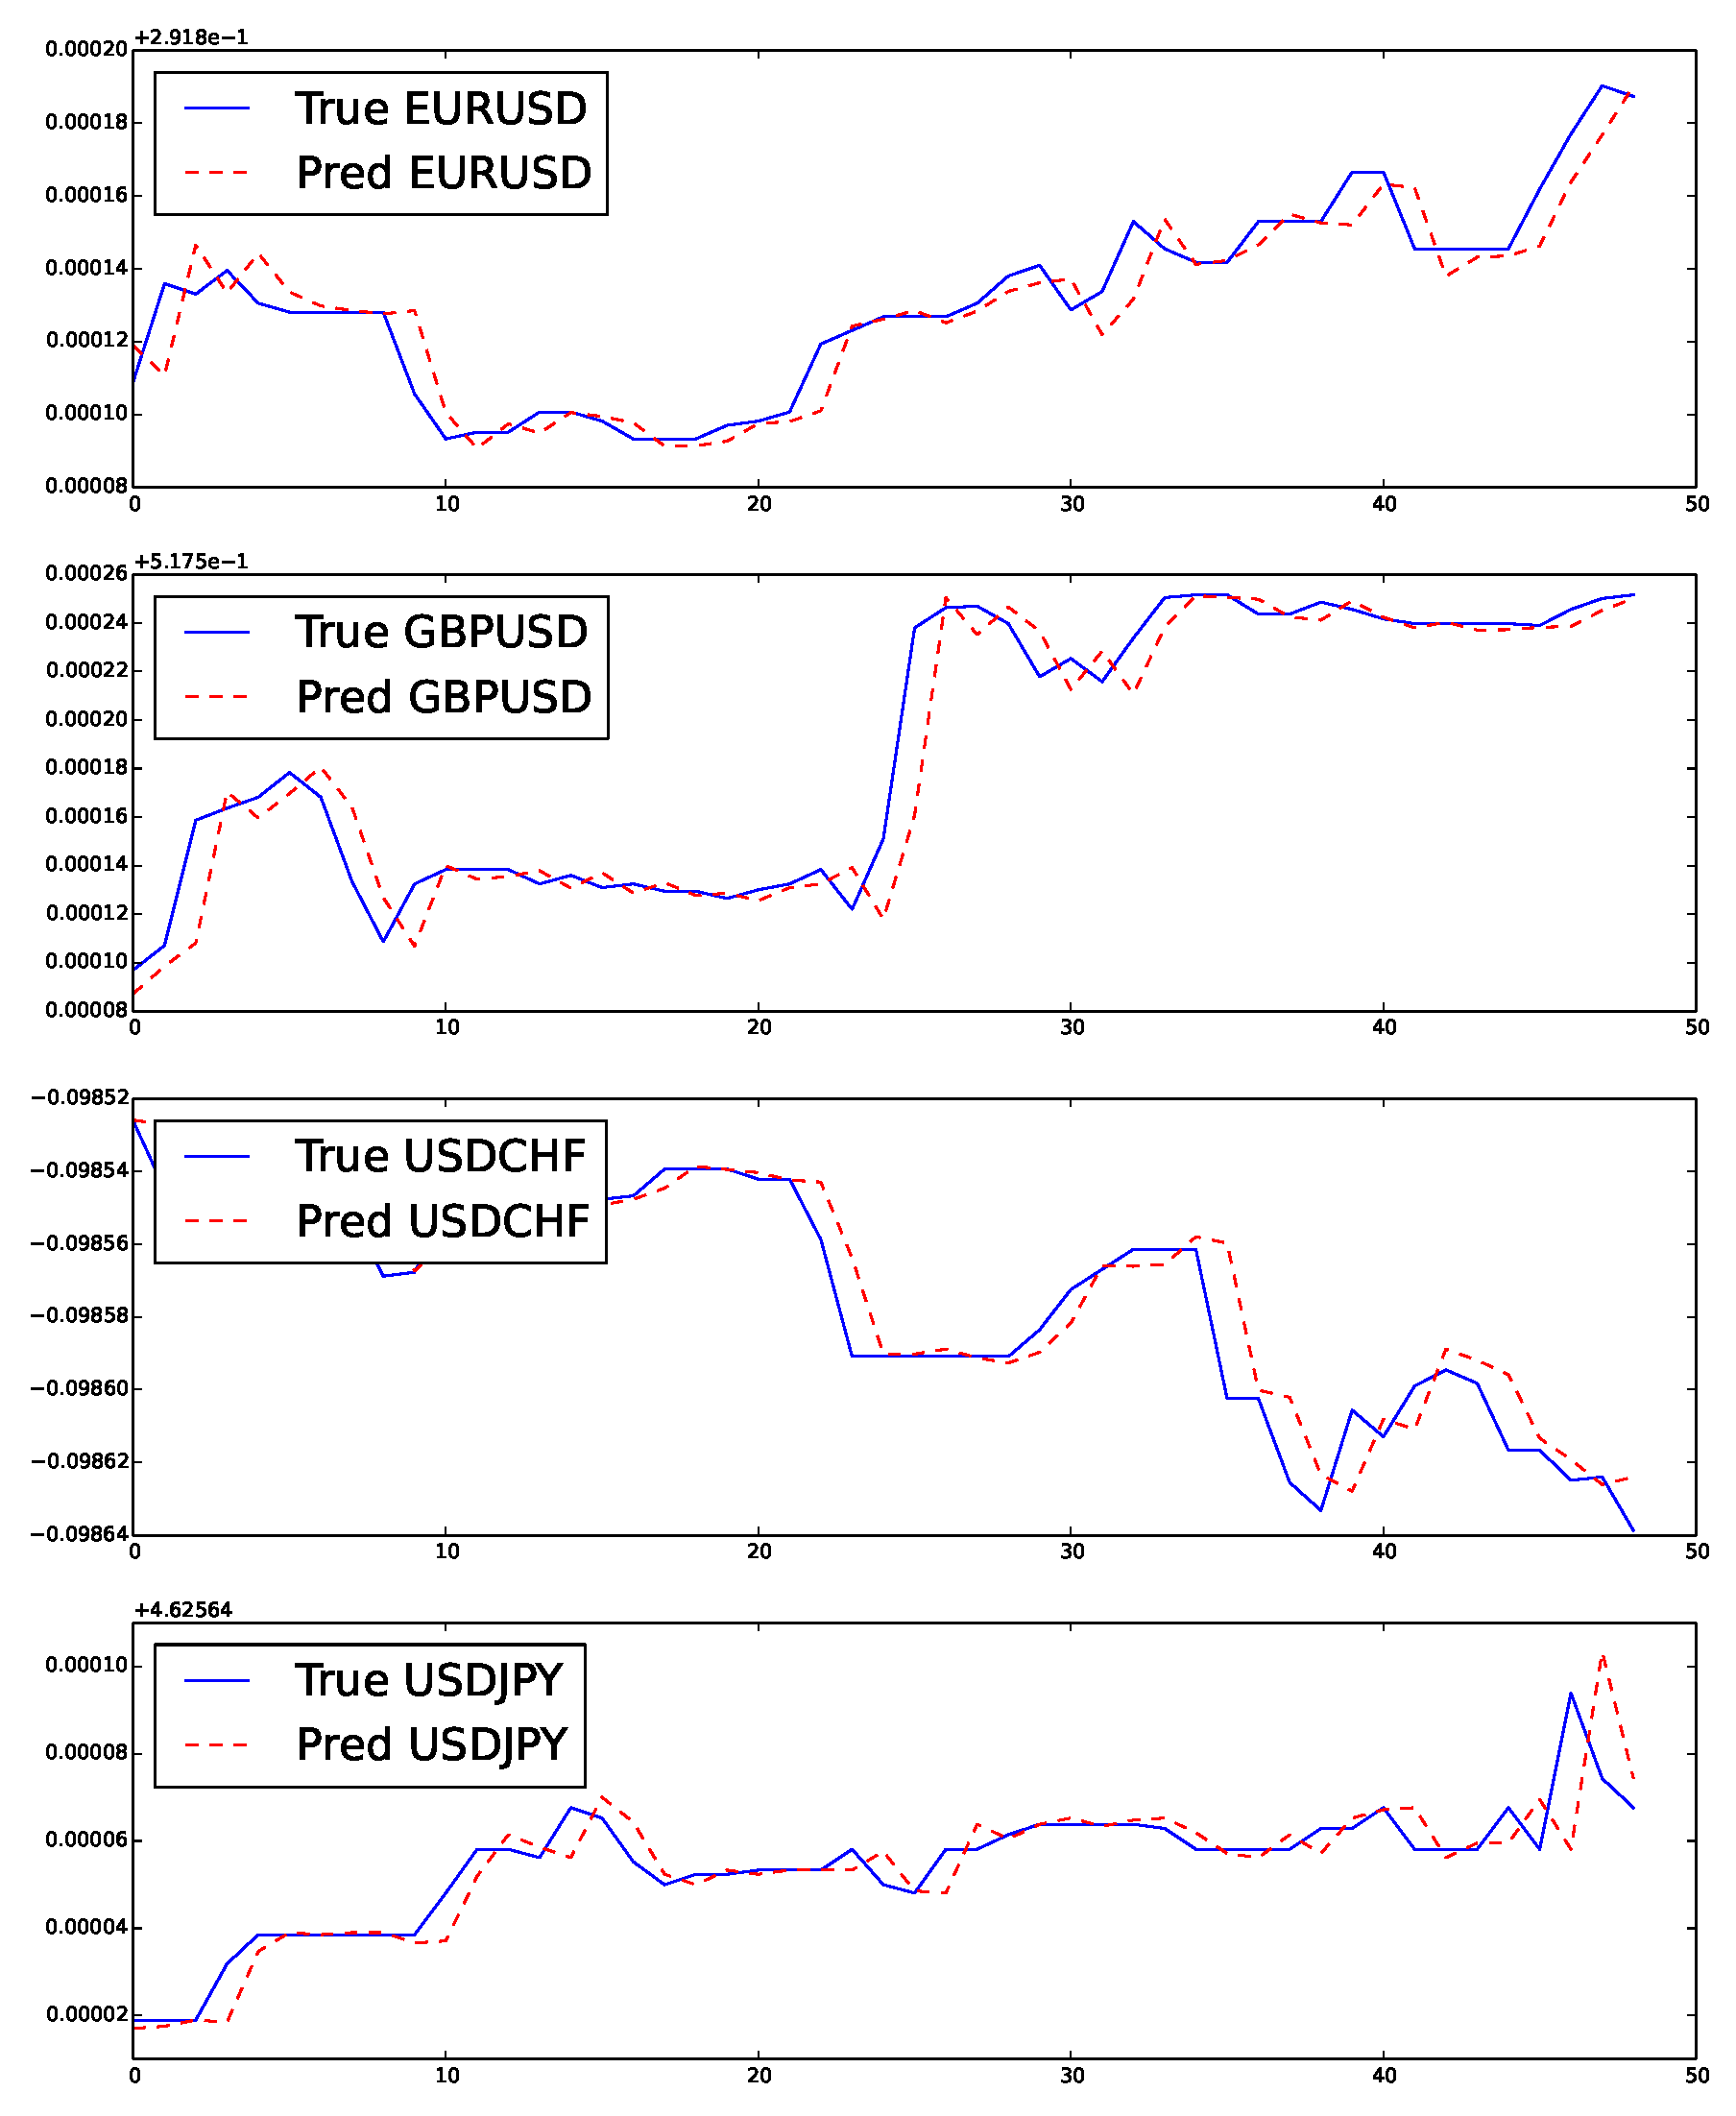
\includegraphics[width = 6cm]{img/accuracy} 
%  \caption{OVECM forecasting accuracy example for 50 minutes using $L = 1000$ and $p =3$}
%  \label{fig:accuracy}
% \end{figure}
%\end{frame}

\section{Conclusions}
\begin{frame}
\frametitle{Conclusions}
\begin{itemize}
\item  OVECM considerably reduces execution times
without compromising solution accuracy.  
\item OVECM was compared with VECM and ARIMA
with the same sliding window sizes and OVECM outperformed both in terms of
execution time. 
\item Traditional VECM slightly outperformed our proposal but the
OVECM execution time is lower.
\item We could see that our algorithm took much less than a minute at every
step. This means that it could also be used with higher frequency data and would
still provide responses before new data arrives.  
\end{itemize}
\end{frame}

\begin{frame}[plain,c]
%\frametitle{A first slide}

\begin{center}
\Huge Thank you for your attention
\Huge Questions?
\end{center}

\end{frame}
\end{document}



